\chapter{Time Series Classification Architectures}
\label{ch:series-architectures}

\begin{figure}[h]
    \centering
    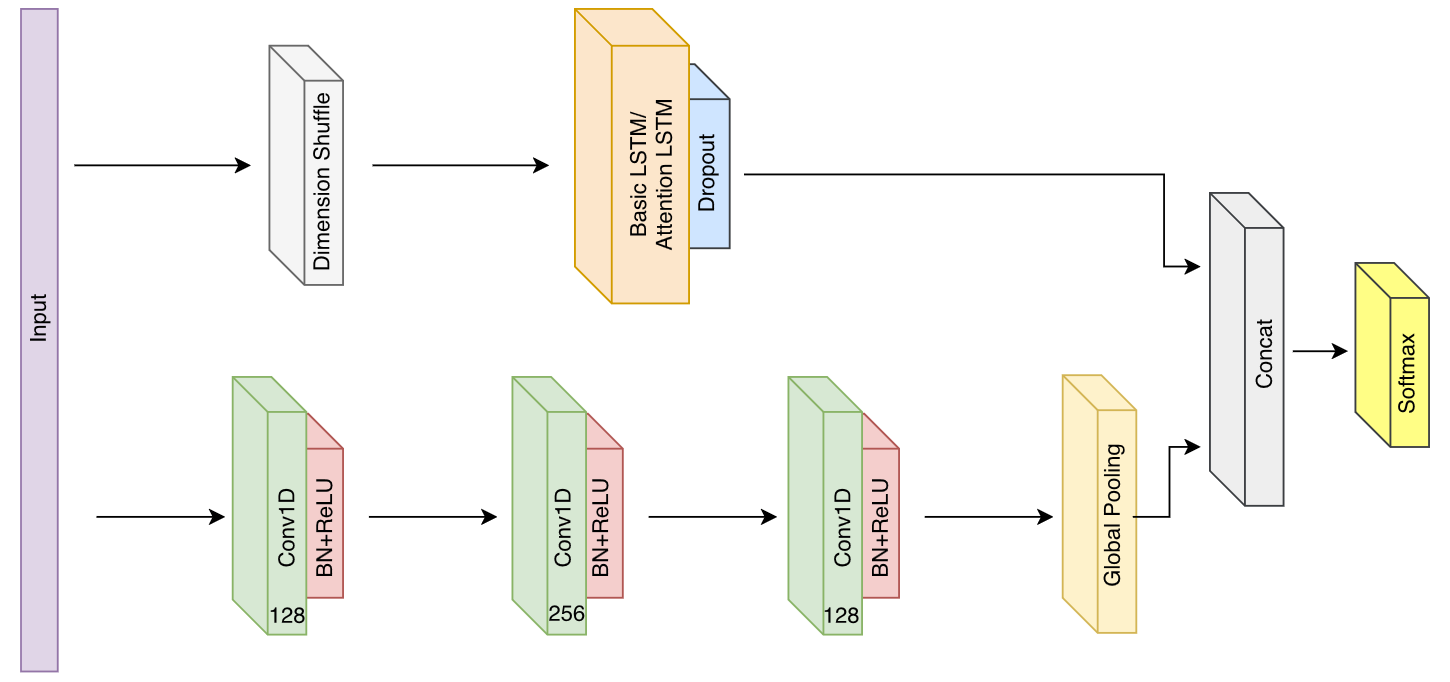
\includegraphics[width=0.75\linewidth]{dissertation//figures/lstm-fcn.png}
    \caption{Architecture for LSTM-FCN architecture\cite{karim2017lstm}}
    \label{fig:lstm-fcn}
\end{figure}

\chapter{Traditional Classification Architectures}
\label{ch:trad-architectures}

\chapter{Deep Fake Detection Challenge Website}
\label{ch:dfdcai}

\begin{figure}[h]
    \centering
    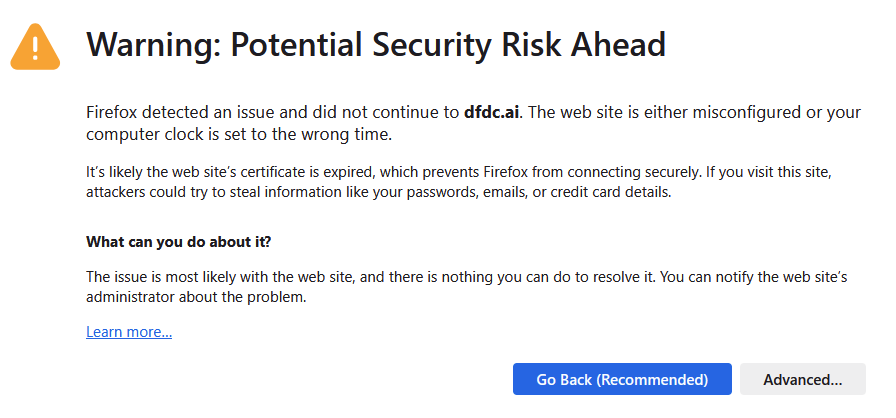
\includegraphics[width=1\linewidth]{dissertation//figures/dfdc.png}
    \caption{A screenshot of the security warning found when trying to access \url{https://dfdc.ai/}}
    \label{fig:dfdcai}
\end{figure}

\chapter{Raw results}
\label{ch:raw-results}

True Positives: declared real when real\\
True Negatives: declared fake when fake\\
False Positives: declared real when fake\\
False Negatives: declared fake when real

\section{Proof of Concept}

\begin{table}[h]
    \centering
    \begin{tabular}{| c | c | c | c | c | c | c |}
        \hline
        \multirow{2}{*}{} & \multicolumn{3}{c|}{\textbf{Unperturbed}} & \multicolumn{3}{c|}{\textbf{Perturbed (VGG, $\epsilon=0.1$)}} \\
        \cline{2-7}
        & \textbf{Blink Detection} & \textbf{VGG} & \textbf{ResNet} & \textbf{Blink Detection} & \textbf{VGG} & \textbf{ResNet} \\
        \hline
        True Positives & 44 & 48 & 45 & 44 & 48 & 45 \\
        \hline
        True Negatives & 36 & 50 & 46 & 32 & 0 & 50 \\
        \hline
        False Positives & 14 & 0 & 4 & 18 & 50 & 0 \\
        \hline
        False Negatives & 6 & 2 & 5 & 6 & 2 & 5 \\
        \hline
        Overall Accuracy & 80\% & 98\% & 91\% & 76\% & 45\% & 95\% \\
        \hline
        Fake Accuracy & 72\% & 100\% & 92\% & 64\% & 0\% & 100\% \\
        \hline
    \end{tabular}
    \caption{Results of the proof of concept}
\end{table}

For unperturbed videos, 1 real video and 27 fake videos were classed as unknown. For perturbed videos, 1 real and 18 fake videos were classed as unknown.  

\section{Main Code}

\subsection{FaceForensics}

The time series analysis paired with HRNet was the time series forest.\\
The time series analysis paired with PFLD was learning shapelets.

\begin{table}[H]
    \centering
    \begin{tabular}{|c|c|c|c|c|c|c|}
        \hline
        \textbf{} & \textbf{HRNet} & \textbf{PFLD} &  \textbf{VGG} & \textbf{ResNet} & \textbf{Xception} & \textbf{EfficientNet} \\
        \hline
        True Positives & 113 & 146 & 175 & 182 & 184 & 176\\
        \hline
        True Negatives & 1672 & 2007 & 2813 & 3035 & 2725 & 2889\\
        \hline
        False Positives & 1528 & 1193 & 387 & 165 & 475 & 311\\
        \hline
        False Negatives & 87 & 54 & 25 & 18 & 16 & 24\\
        \hline
        Overall Accuracy & 52.5\% & 63.3\% & 87.9\% & 94.6\% & 85.6\% & 90.1\% \\
        \hline
        Fake Accuracy & 52.3\% & 62.7\% & 87.9\% & 94.8\% & 85.2\% & 90.3\% \\
        \hline
    \end{tabular}
    \caption{Unperturbed}
\end{table}

\begin{table}[H]
    \centering
    \begin{tabular}{|c|c|c|c|c|c|c|}
        \hline
        \textbf{} & \textbf{HRNet} & \textbf{PFLD} &  \textbf{VGG} & \textbf{ResNet} & \textbf{Xception} & \textbf{EfficientNet} \\
        \hline
        True Negatives & 1683 & 2006 & 9 & 486 & 541 & 1069\\
        \hline
        False Positives & 1517 & 1194 & 3191 & 2714 & 2659 & 2131\\
        \hline
        Accuracy & 52.6\% & 62.7\% & 0.2\% & 15.2\% & 16.9\% & 33.4\% \\
        \hline
    \end{tabular}
    \caption{Perturbed (VGG, $\epsilon=0.05$)}
\end{table}

\begin{table}[H]
    \centering
    \begin{tabular}{|c|c|c|c|c|c|c|}
        \hline
        \textbf{} & \textbf{HRNet} & \textbf{PFLD} &  \textbf{VGG} & \textbf{ResNet} & \textbf{Xception} & \textbf{EfficientNet} \\
        \hline
        True Negatives & 1730 & 2006 & 0 & 155 & 1086 & 1972\\
        \hline
        False Positives & 1470 & 1194 & 3200 & 3045 & 2114 & 1228\\
        \hline
        Accuracy & 54.1\% & 62.7\% & 0\% & 4.8\% & 33.9\% & 61.6\% \\
        \hline
    \end{tabular}
    \caption{Perturbed (VGG, $\epsilon = 0.1$)}
\end{table}

\begin{table}[H]
    \centering
    \begin{tabular}{|c|c|c|c|c|c|c|}
        \hline
        \textbf{} & \textbf{HRNet} & \textbf{PFLD} &  \textbf{VGG} & \textbf{ResNet} & \textbf{Xception} & \textbf{EfficientNet} \\
        \hline
        True Negatives & 1671 & 2005 & 605 & 0 & 507 & 992\\
        \hline
        False Positives & 1529 & 1195 & 2595 & 3200 & 2693 & 2208\\
        \hline
        Accuracy & 52.2\% & 62.7\% & 18.9\% & 0\% & 15.6\% & 31\% \\
        \hline
    \end{tabular}
    \caption{Perturbed (ResNet, $\epsilon=0.05$)}
\end{table}

\begin{table}[H]
    \centering
    \begin{tabular}{|c|c|c|c|c|c|c|}
        \hline
        \textbf{} & \textbf{HRNet} & \textbf{PFLD} &  \textbf{VGG} & \textbf{ResNet} & \textbf{Xception} & \textbf{EfficientNet} \\
        \hline
        True Negatives & 1716 & 2007 & 33 & 0 & 1107 & 1966\\
        \hline
        False Positives & 1484 & 1993 & 3167 & 3200 & 2093 & 1234\\
        \hline
        Accuracy & 53.6\% & 62.7\% & 1\% & 0\% & 34.6\% & 61.4\% \\
        \hline
    \end{tabular}
    \caption{Perturbed (ResNet, $\epsilon=0.1$)}
\end{table}

\begin{table}[H]
    \centering
    \begin{tabular}{|c|c|c|c|c|c|c|}
        \hline
        \textbf{} & \textbf{HRNet} & \textbf{PFLD} &  \textbf{VGG} & \textbf{ResNet} & \textbf{Xception} & \textbf{EfficientNet} \\
        \hline
        True Negatives & 1681 & 2007 & 497 & 267 & 2 & 924\\
        \hline
        False Positives & 1519 & 1193 & 2703 & 2933 & 3198 & 2276\\
        \hline
        Accuracy & 52.5\% & 62.7\% & 15.5\% & 8.3\% & 0\% & 28.9\% \\
        \hline
    \end{tabular}
    \caption{Perturbed (Xception, $\epsilon=0.05$)}
\end{table}

\begin{table}[H]
    \centering
    \begin{tabular}{|c|c|c|c|c|c|c|}
        \hline
        \textbf{} & \textbf{HRNet} & \textbf{PFLD} &  \textbf{VGG} & \textbf{ResNet} & \textbf{Xception} & \textbf{EfficientNet} \\
        \hline
        True Negatives & 1699 & 2007 & 27 & 178 & 1 & 1921\\
        \hline
        False Positives & 1501 & 1193 & 3173 & 3022 & 3199 & 1279 \\
        \hline
        Accuracy & 53.1\% & 62.6\% & 0.1\% & 5.6\% & 0\% & 60\% \\
        \hline
    \end{tabular}
    \caption{Perturbed (Xception, $\epsilon=0.1$)}
\end{table}

\begin{table}[H]
    \centering
    \begin{tabular}{|c|c|c|c|c|c|c|}
        \hline
        \textbf{} & \textbf{HRNet} & \textbf{PFLD} &  \textbf{VGG} & \textbf{ResNet} & \textbf{Xception} & \textbf{EfficientNet} \\
        \hline
        True Negatives & 1673 & 2006 & 605 & 425 & 537 & 0\\
        \hline
        False Positives & 1527 & 1194 & 2595 & 2775 & 2663 & 3200\\
        \hline
        Accuracy & 52.3\% & 62.7\% & 18.9\% & 13.3\% & 16.8\% & 0\% \\
        \hline
    \end{tabular}
    \caption{Perturbed (EfficientNet, $\epsilon=0.05$)}
\end{table}

\begin{table}[H]
    \centering
    \begin{tabular}{|c|c|c|c|c|c|c|}
        \hline
        \textbf{} & \textbf{HRNet} & \textbf{PFLD} &  \textbf{VGG} & \textbf{ResNet} & \textbf{Xception} & \textbf{EfficientNet} \\
        \hline
        True Negatives & 1722 & 2008 & 33 & 134 & 1085 & 0\\
        \hline
        False Positives & 1478 & 1992 & 3167 & 3066 & 2115 & 3200\\
        \hline
        Accuracy & 53.8\% & 62.8\% & 1\% & 4.2\% & 33.9\% & 0\% \\
        \hline
    \end{tabular}
    \caption{Perturbed (EfficientNet, $\epsilon=0.1$)}
\end{table}

\subsection{Celeb-DF}

The time series analysis paired with HRNet was learning shapelets.\\
The time series analysis paired with PFLD was learning shapelets.

\begin{table}[H]
    \centering
    \begin{tabular}{|c|c|c|c|c|c|c|}
        \hline
        \textbf{} & \textbf{HRNet} & \textbf{PFLD} &  \textbf{VGG} & \textbf{ResNet} & \textbf{Xception} & \textbf{EfficientNet} \\
        \hline
        True Positives & 103 & 104 & 165 & 174 & 172 & 171\\
        \hline
        True Negatives & 3021 & 2930 & 4838 & 4896 & 4833 & 4877\\
        \hline
        False Positives & 1906 & 1997 & 89 & 31 & 94 & 50\\
        \hline
        False Negatives & 75 & 74 & 13 & 4 & 6 & 7\\
        \hline
        Overall Accuracy & 61.2\% & 59.4\% & 98\% & 99.3\% & 98\% & 98.9\% \\
        \hline
        Fake Accuracy & 61.3\% & 59.5\% & 98.2\% & 99.4\% & 98.1\% & 99\% \\
        \hline
    \end{tabular}
    \caption{Unperturbed}
\end{table}

\begin{table}[H]
    \centering
    \begin{tabular}{|c|c|c|c|c|c|c|}
        \hline
        \textbf{} & \textbf{HRNet} & \textbf{PFLD} &  \textbf{VGG} & \textbf{ResNet} & \textbf{Xception} & \textbf{EfficientNet} \\
        \hline
        True Negatives &  & 2937 & 0 & 4040 & 4647 & 486\\
        \hline
        False Positives &  & 1990 & 4927 & 887 & 280 & 4441\\
        \hline
        Accuracy & \% & 59.6\% & 0\% & 82\% & 94.3\% & 9.9\% \\
        \hline
    \end{tabular}
    \caption{Perturbed (VGG, $\epsilon=0.05$)}
\end{table}

\begin{table}[H]
    \centering
    \begin{tabular}{|c|c|c|c|c|c|c|}
        \hline
        \textbf{} & \textbf{HRNet} & \textbf{PFLD} &  \textbf{VGG} & \textbf{ResNet} & \textbf{Xception} & \textbf{EfficientNet} \\
        \hline
        True Negatives & 3021 & 2952 & 0 & 4927 & 3754 & 4\\
        \hline
        False Positives & 1906 & 1957 & 4927 & 0 & 1173 & 4923\\
        \hline
        Accuracy & 61.3\% & 59.9\% & 0\% & 100\% & 76.2\% & 0.1\% \\
        \hline
    \end{tabular}
    \caption{Perturbed (VGG, $\epsilon = 0.1$)}
\end{table}

\begin{table}[H]
    \centering
    \begin{tabular}{|c|c|c|c|c|c|c|}
        \hline
        \textbf{} & \textbf{HRNet} & \textbf{PFLD} &  \textbf{VGG} & \textbf{ResNet} & \textbf{Xception} & \textbf{EfficientNet} \\
        \hline
        True Negatives &  & 2939 & 215 & 0 & 4582 & 414\\
        \hline
        False Positives &  & 1988 & 4712 & 4927 & 345 & 4513\\
        \hline
        Accuracy & \% & 59.7\% & 4.3\% & 0\% & 93\% & 8.4\% \\
        \hline
    \end{tabular}
    \caption{Perturbed (ResNet, $\epsilon=0.05$)}
\end{table}

\begin{table}[H]
    \centering
    \begin{tabular}{|c|c|c|c|c|c|c|}
        \hline
        \textbf{} & \textbf{HRNet} & \textbf{PFLD} &  \textbf{VGG} & \textbf{ResNet} & \textbf{Xception} & \textbf{EfficientNet} \\
        \hline
        True Negatives & 3021 & 2952 & 103 & 3357 & 3724 & 3\\
        \hline
        False Positives & 1906 & 1975 & 4824 & 1570 & 1203 & 4924\\
        \hline
        Accuracy & 61.3\% & 59.9\% & 2.1\% & 68.1\% & 75.6\% & 0.1\% \\
        \hline
    \end{tabular}
    \caption{Perturbed (ResNet, $\epsilon=0.1$)}
\end{table}

\begin{table}[H]
    \centering
    \begin{tabular}{|c|c|c|c|c|c|c|}
        \hline
        \textbf{} & \textbf{HRNet} & \textbf{PFLD} &  \textbf{VGG} & \textbf{ResNet} & \textbf{Xception} & \textbf{EfficientNet} \\
        \hline
        True Negatives &  & 2936 & 193 & 3323 & 2 & 134\\
        \hline
        False Positives &  & 1991 & 4734 & 1604 & 4925 & 4793\\
        \hline
        Accuracy & \% & 59.6\% & 3.9\% & 67.4\% & 0\% & 2.7\% \\
        \hline
    \end{tabular}
    \caption{Perturbed (Xception, $\epsilon=0.05$)}
\end{table}

\begin{table}[H]
    \centering
    \begin{tabular}{|c|c|c|c|c|c|c|}
        \hline
        \textbf{} & \textbf{HRNet} & \textbf{PFLD} &  \textbf{VGG} & \textbf{ResNet} & \textbf{Xception} & \textbf{EfficientNet} \\
        \hline
        True Negatives & 3021 & 2951 & 96 & 4927 & 0 & 3\\
        \hline
        False Positives & 1906 & 1976 & 4831 & 0 & 4927 & 4924\\
        \hline
        Accuracy & 61.3\% & 59.9\% & 1.9\% & 100\% & 0\% & 0\% \\
        \hline
    \end{tabular}
    \caption{Perturbed (Xception, $\epsilon=0.1$)}
\end{table}

\begin{table}[H]
    \centering
    \begin{tabular}{|c|c|c|c|c|c|c|}
        \hline
        \textbf{} & \textbf{HRNet} & \textbf{PFLD} &  \textbf{VGG} & \textbf{ResNet} & \textbf{Xception} & \textbf{EfficientNet} \\
        \hline
        True Negatives &  & 2938 & 215 & 3955 & 4580 & 0\\
        \hline
        False Positives &  & 1988 & 4712 & 972 & 347 & 4927\\
        \hline
        Accuracy & \% & 59.6\% & 4.4\% & 80.3\% & 93\% & 0\% \\
        \hline
    \end{tabular}
    \caption{Perturbed (EfficientNet, $\epsilon=0.05$)}
\end{table}

\begin{table}[H]
    \centering
    \begin{tabular}{|c|c|c|c|c|c|c|}
        \hline
        \textbf{} & \textbf{HRNet} & \textbf{PFLD} &  \textbf{VGG} & \textbf{ResNet} & \textbf{Xception} & \textbf{EfficientNet} \\
        \hline
        True Negatives & 3021 & 2952 & 96 & 4927 & 0 & 3\\
        \hline
        False Positives & 1906 & 1975 & 4831 & 0 & 4927 & 4924\\
        \hline
        Accuracy & 61.3\% & 59.9\% & 1.9\% & 100\% & 0\% & 0\% \\
        \hline
    \end{tabular}
    \caption{Perturbed (EfficientNet, $\epsilon=0.1$)}
\end{table}

\section{Transferability}

\begin{table}[H]
    \centering
    \begin{tabular}{|c|c|c|c|c|c|c|}
        \hline
        \textbf{} & \textbf{HRNet} & \textbf{PFLD} & \textbf{VGG} & \textbf{ResNet} & \textbf{Xception} & \textbf{EfficientNet} \\
        \hline
        True Positives &  &  &  &  &  & \\
        \hline
        True Negatives &  &  &  &  &  & \\
        \hline
        False Positives &  &  &  &  &  & \\
        \hline
        False Negatives &  &  &  &  &  & \\
        \hline
        Overall Accuracy & \% & \% & \% & \% & \% & \% \\
        \hline
        Fake Accuracy & \% & \% & \% & \% & \% & \% \\
        \hline
    \end{tabular}
    \caption{The accuracy of models trained on FaceForensics and tested on FakeAVCeleb}
\end{table}

\begin{table}[H]
    \centering
    \begin{tabular}{|c|c|c|c|c|c|c|}
        \hline
        \textbf{} & \textbf{HRNet} & \textbf{PFLD} & \textbf{VGG} & \textbf{ResNet} & \textbf{Xception} & \textbf{EfficientNet} \\
        \hline
        True Positives &  &  &  &  &  & \\
        \hline
        True Negatives &  &  &  &  &  & \\
        \hline
        False Positives &  &  &  &  &  & \\
        \hline
        False Negatives &  &  &  &  &  & \\
        \hline
        Overall Accuracy & \% & \% & \% & \% & \% & \% \\
        \hline
        Fake Accuracy & \% & \% & \% & \% & \% & \% \\
        \hline
    \end{tabular}
    \caption{The accuracy of models trained on Celeb DeepFake and tested on FakeAVCeleb}
\end{table}

\chapter{Open Source Contributions}